\chapter{Evaluating the results}
\label{chapter:evaluation}

%You have done your work, but that's\footnote{By the way, do \emph{not} use
%shorthands like this in your text! It is not professional! Always write out all
%the words: ``that is''.} not enough. 

%You also need to evaluate how well your implementation works.  The
%nature of the evaluation depends on your problem, your method, and
%your implementation that are all described in the thesis before this
%chapter.  If you have created a program for exact-text matching, then
%you measure how long it takes for your implementation to search for
%different patterns, and compare it against the implementation that was
%used before.  If you have designed a process for managing software
%projects, you perhaps interview people working with a waterfall-style
%management process, have them adapt your management process, and
%interview them again after they have worked with your process for some
%time. See what's changed.

%The important thing is that you can evaluate your success somehow.
%Remember that you do not have to succeed in making something spectacular; a
%total implementation failure may still give grounds for a very good master's
%thesis---if you can analyze what went wrong and what should have been
%done. 

 %At this point, you will have some insightful thoughts on your
%implementation and you may have ideas on what could be done in the
%future. This chapter may be combined together with the evaluation
%chapter. All the new insights and findings are given here!  This
%chapter is a good place to discuss your thesis as a whole and to show
%your professor that you have really understood some non-trivial
%aspects of the methods you used\ldots

In this final chapter before conclusion, we will be examining the pipeline which we build in the previous chapter.
We start with basic perfomance metrics that were briefly introduced in the section 4.4.
Then we move on to qualitive metrics and questions that we also defined in the section 4.4 and discuss about the pipeline using them.
We then move to examine general flaws in this study to give more complete image of the results and follow this by reflection on what could have been possibly done better and why some detrimental choices were made. 
Finally we close this chapter with a section were we briefly list possible improvements that could improve the current pipeline, but could not be implemented with the resource and time restrictions that this project had.

\section{Perfomance metrics}

We start by defining the environment where the following results were derived.
The following metrics were taken in a machine that has a Windows 10 as parent operating system, Intel Core i5 2500K processor and 16GB of DDR3 memory.
The docker version that the code was run against was 19.03.2 and it had 3 CPU cores and 10GB of memory as its use.
Not all of these resources were needed, but this was done to in order to remove the factors of running out of memory that could cause inexplicable errors.
These were tested only in one machine which would usually not be enough to make any kind of actual inferences but because the code is run in a containerized environment the role of underlying hardware becomes less important.

\begin{figure}[ht!]
    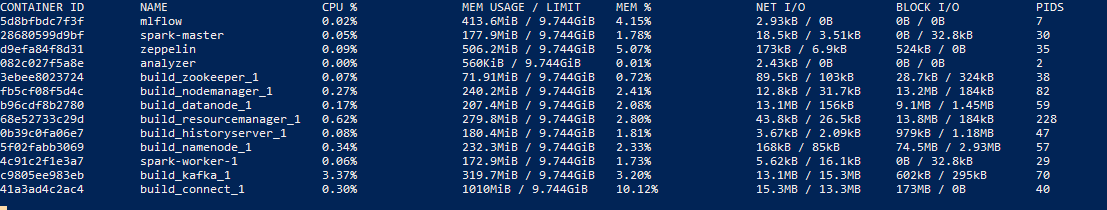
\includegraphics[scale=0.45]{images/memory1} 
    \centering
    \caption{Resource usage in idle state}
\end{figure}

The resource usage in idle state after the initial data has gone through the pipeline and stored into HDFS can be seen in the figure 6.1.
The figure is the output of the "docker stats" -command.
While inspecting the names of each container the reader should be able to map these into corresponding components in the architechture figure in section 5.2, but to clarify the most ambigous namings, the "analyzer" container refers to the standalone DL4J application and build\_connect\_1 refers to the Kafka Connect instance.

The total memory usage here was around 3.8GiB.
This seems to match with the fact that most of the components ran on top JVM and we did not have the time to optimize each components garbage collection. 
This is partly because components such as the Kafka Connect, which had a notably large memory usage, would silently fail if not enough memory were offered.
Additionally, this would have probably lead to premature optimization.
For future improvements on the accessibility of the pipeline, this would be a great place to start.

Processor usage in idle state was minimal and did not have any notable jumps except a bit higher usage for Kafka.
The other statistics did not have any notable deviations that would affect greatly on the usage of the pipeline. 
Minor thing to note is that the DL4J application instance is not running actively during these results as user usually are not using both it and the zeppelin instances simultaneously.

\begin{figure}[ht!]
    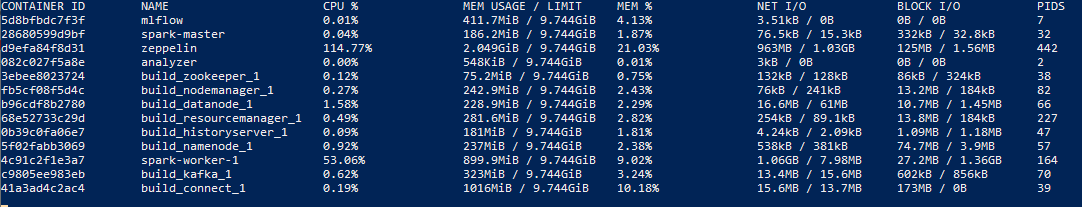
\includegraphics[scale=0.45]{images/memory2} 
    \centering
    \caption{Resource usage in preprocessing state}
\end{figure}

In figure 6.2 we have the same statistics while the zeppelin code is trying to preprocess the data in order to feed it into LSTM network.
The pipeline has at this point run for some time and the overall memory load has increased to 6.1GiB.
This is mainly due to Zeppelin and Spark worker using a lot more memory.
The CPU usage for both has raised, and one can see that at the moment of taking these stats the notebook code is actually using more resources than the actual worker.

As there was not enough time to test other technologies in pipeline these results by themselves do not give us much information about the quality of the software.
They do give us some information about the requirements of the machine that is needed to run locally a pipeline that is this complex.
Over 8GiB of memory is almost a must to run it in active use where the data is flowing continously.
The need for memory can be alleviated with proper garbage collection, but peak memory usage can reach to these numbers.

\section{Pipeline management}

The main benefits of this pipeline do not come from its perfomance.
It is highly containerized meaning it can run with little to none re-configuration on any machine.
During the development of this pipeline the pipeline was developed first on Mac OS and then because of memory requirements moved to Windows machine.
The porting of code did not require any extra steps, other than making sure that the formating of line endings stayed the same with script files that are run in containerized linux environment.

Docker containers also allow the development in isolated networked environment that is very similar to one which would be used in production.
This means that most of the problems that could occur when rolling locally developed code into a production environment where services lie on different machine interconnected by a network, are already solved in here before the user has even started development.
Only thing that the user has to do is to change the addresses in this code from docker based DNS to the addresses used in their own cloud environment.

As explained earlier, the technologies such as Kafka Connect have been chosen so that changing one techonology does not have large impacts on the overall architecture.
If the user would want to change some component in the pipeline, the integrations between components have to be done again but this has been made as easy as possible.

The pipeline is also mostly automated.
No manual input is required from the user to setup the basic pipeline which makes adapting the pipeline quite trivial.
Only in the analysis phase, users manual input is needed to control the pipeline.

Machine Learning pipeline monitoring is made easy with MLFlow.
Although logging new experiments needs a bit of manual work for user because of the nature of MLFlow API, but nevertheless it does make managing the machine learning models easier.
The only downside here is that by default MLFlow does not yet accept DL4J models to be saved in its containerized packages which would make model export easier.

For general monitoring the pipeline is still lacking because we did not have time to implement the ELK stack.
Almost each component has its own monitoring UI but these are scattered making it hard to follow the bigger picture of the pipeline which was one of the problems we introduced in the chapter 2.
The exception of not having an own monitoring UI is the Kafka Connect.
It offers REST API to monitor its metrics which would need additional integration with some log monitoring solution such as ELK.

\section{Flaws in the end product}

In this section we examine general flaws in the pipeline that we are aware of.
We try to objectively examine these and try to give some reasoning why these flaws did happen and how they could be fixed.
We will leave out here the flaws in monitoring as these were mostly examined in the previous section.

Currently, the main method of training machine learning models is to use computers graphics card (GPU) which is multiple times faster than using CPUs.
This makes the current pipeline vastly underperforming when it comes to training machine learning models and this is a clear downside for this system.
It needs quite a bit of CPUs and good networking before it even reaches the perfomance of a single high-end GPU.
The DL4J, does however, support GPU training on spark cluster meaning that adding GPU support to this pipeline with small amount of work is possible.
However, we did not have time to implement it as it needs some work for docker to access CUDA resources on parent OS.

Unfortunately, because we were only able to try the HDFS as the storage method, the storage is currently lacking a proper query properties meaning that the user has to pull the entire timeseries for each stock.
This in big data context is not desirable behaviour, but integrating a technology like HBase should not need much additional work.
However, for us it is already out of the scope of this project.

With the resources this project had, the pipeline could not be tested with actual complete stock market data, which leaves means that we have no prove that the pipeline actually can scale with the data or if this scaling is even possible with the pipeline.
We can only speculate this based on the each of technologies abilities but the possibility for horizontal scalability should be there theoretically.

\section{Reflection}

In this section we will reflect back on the implementation part and discuss what possibly went wrong on the development of the pipeline.
We will try our best to explain the choices taken while being aware that there could have been better alternatives.

Choosing DL4J as the machine learning library turned out to be a time consuming option.
After the implementation part, it was clear why data scientist usually use python libraries such as Keras and PyTorch, the amount of resources is substantially larger.
Many of the problems faced during development had quite simple solutions to them, but they were really hard to solve without any reference and empty search results on Google.
This combined with the out-of-date examples lead to problems seen in the previous chapter.

One can question whetever we should have opted out from DL4J during development and changed it to some other more compatible library.
We did not do this because there was not that many sensible choices and the documentation and resources online of those that seemed promising were even worse than with the DL4J.
But although the original plan to build to multiple pipelines was not possible partly because of this, we think that the information produced in the implementation chapter is quite valuable on its own and can help a lot of developers who have restrictions on what technologies they can use.

Of course, the scope of the implementation part could have been narrowed down as it was quite ambigous.
Especially, during development things that seemed simple turned out to be quite more complex than initially thought.
The inexperience about some of the technologies used did affect the results, but it also indicates that the documentation of some technologies could have been better.
Quite a bit of things were assumed in the documentations, which lead to errors that probably could not had happened with right documentation.

\section{Potential improvements}

There are quite a bit of improvements already mentioned at the previous sections as these usually are part of the problems, but we have gathered them and a couple others to this section to give a clearer view on what could be improved.
These are quite straightforward to implement but implementing them can take some time.

As stated before, the perfomance of the pipeline could be improved.
This could be done by adding support for GPU usage in Spark cluster which would require the configuration of docker to give the process access to these.
Memory usage could be probably optimized by configuring better carbage collection on components that take most of the memory.

To make the pipeline more automated and improve its mobility, urls for servers could be made dynamic with for example environmental variables that could be configured by the user.
Other such configurations could be made in order to make porting the code to a different environment easier.

The final giveaway in this chapter is that there was quite a bit of things that could have been done better. 
This is partly because of the ambigious scope of the project, inexperience of the author and lack of correct information online.
Despite these, we think that the complications during the development and the final product do offer valuable insights on developing a pipeline for stock data analysis using these technologies and can give somebody a basis to start developing their own pipeline.
Now we move on to the final chapter where we conclude and summarize everything that we have learned during this thesis.